\XtoCBlock{Real2Int}
\label{block:Real2Int}
\begin{figure}[H]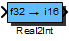
\includegraphics{Real2Int}\end{figure} 

\begin{XtoCtabular}{Inports}
In & Real input\tabularnewline
\hline
\end{XtoCtabular}


\begin{XtoCtabular}{Outports}
Out & Integer output\tabularnewline
\hline
\end{XtoCtabular}

\begin{XtoCMaskParamTabular}{Mask Parameters}
\rowcolor[gray]{0.8}\textbf{Name} & \textbf{ID} & \textbf{Description}\tabularnewline\hline
Scale & 1 & Scaling factor from real to integer\tabularnewline
\hline
\end{XtoCMaskParamTabular}

\subsubsection*{Description:}
Conversion block from real (floating point) datatypes to integer (fixed point) datatypes.

  Out = In / Scale 

% include optional documentation file
\InputIfFileExists{\XcHomePath/Library/General/Doc/Real2Int_Info.tex}{\vspace{1ex}}{}

\subsubsection*{Implementations:}
\begin{tabular}{l l}
\textbf{Float32\_FiP8} & 32 Floating Point to 8 Bit Fixed Point Implementation\tabularnewline
\textbf{Float32\_FiP16} & 32 Floating Point to 16 Bit Fixed Point Implementation\tabularnewline
\textbf{Float32\_FiP32} & 32 Floating Point to 32 Bit Fixed Point Implementation\tabularnewline
\textbf{Float64\_FiP8} & 64 Floating Point to 8 Bit Fixed Point Implementation\tabularnewline
\textbf{Float64\_FiP16} & 64 Floating Point to 16 Bit Fixed Point Implementation\tabularnewline
\textbf{Float64\_FiP32} & 64 Floating Point to 32 Bit Fixed Point Implementation\tabularnewline
\textbf{Float32\_Bool} & 32 Floating Point to Boolean Implementation\tabularnewline
\textbf{Float64\_Bool} & 64 Floating Point to Boolean Implementation\tabularnewline
\end{tabular}

\XtoCImplementation{Float32\_FiP8}
\nopagebreak[0]

32 Floating Point to 8 Bit Fixed Point Implementation

\begin{XtoCtabular}{Inports Data Type}
In & float32\tabularnewline
\hline
\end{XtoCtabular}

\begin{XtoCtabular}{Outports Data Type}
Out & int8\tabularnewline
\hline
\end{XtoCtabular}

\ifdefined \AddTestReports
\InputIfFileExists{\XcHomePath/Library/General/Doc/Test-Results/Test_Real2Int_Float32_FiP8.tex}{}{}
\fi
\XtoCImplementation{Float32\_FiP16}
\nopagebreak[0]

32 Floating Point to 16 Bit Fixed Point Implementation

\begin{XtoCtabular}{Inports Data Type}
In & float32\tabularnewline
\hline
\end{XtoCtabular}

\begin{XtoCtabular}{Outports Data Type}
Out & int16\tabularnewline
\hline
\end{XtoCtabular}

\ifdefined \AddTestReports
\InputIfFileExists{\XcHomePath/Library/General/Doc/Test-Results/Test_Real2Int_Float32_FiP16.tex}{}{}
\fi
\XtoCImplementation{Float32\_FiP32}
\nopagebreak[0]

32 Floating Point to 32 Bit Fixed Point Implementation

\begin{XtoCtabular}{Inports Data Type}
In & float32\tabularnewline
\hline
\end{XtoCtabular}

\begin{XtoCtabular}{Outports Data Type}
Out & int32\tabularnewline
\hline
\end{XtoCtabular}

\ifdefined \AddTestReports
\InputIfFileExists{\XcHomePath/Library/General/Doc/Test-Results/Test_Real2Int_Float32_FiP32.tex}{}{}
\fi
\XtoCImplementation{Float64\_FiP8}
\nopagebreak[0]

64 Floating Point to 8 Bit Fixed Point Implementation

\begin{XtoCtabular}{Inports Data Type}
In & float64\tabularnewline
\hline
\end{XtoCtabular}

\begin{XtoCtabular}{Outports Data Type}
Out & int8\tabularnewline
\hline
\end{XtoCtabular}

\ifdefined \AddTestReports
\InputIfFileExists{\XcHomePath/Library/General/Doc/Test-Results/Test_Real2Int_Float64_FiP8.tex}{}{}
\fi
\XtoCImplementation{Float64\_FiP16}
\nopagebreak[0]

64 Floating Point to 16 Bit Fixed Point Implementation

\begin{XtoCtabular}{Inports Data Type}
In & float64\tabularnewline
\hline
\end{XtoCtabular}

\begin{XtoCtabular}{Outports Data Type}
Out & int16\tabularnewline
\hline
\end{XtoCtabular}

\ifdefined \AddTestReports
\InputIfFileExists{\XcHomePath/Library/General/Doc/Test-Results/Test_Real2Int_Float64_FiP16.tex}{}{}
\fi
\XtoCImplementation{Float64\_FiP32}
\nopagebreak[0]

64 Floating Point to 32 Bit Fixed Point Implementation

\begin{XtoCtabular}{Inports Data Type}
In & float64\tabularnewline
\hline
\end{XtoCtabular}

\begin{XtoCtabular}{Outports Data Type}
Out & int32\tabularnewline
\hline
\end{XtoCtabular}

\ifdefined \AddTestReports
\InputIfFileExists{\XcHomePath/Library/General/Doc/Test-Results/Test_Real2Int_Float64_FiP32.tex}{}{}
\fi
\XtoCImplementation{Float32\_Bool}
\nopagebreak[0]

32 Floating Point to Boolean Implementation

\begin{XtoCtabular}{Inports Data Type}
In & float32\tabularnewline
\hline
\end{XtoCtabular}

\begin{XtoCtabular}{Outports Data Type}
Out & bool\tabularnewline
\hline
\end{XtoCtabular}

\ifdefined \AddTestReports
\InputIfFileExists{\XcHomePath/Library/General/Doc/Test-Results/Test_Real2Int_Float32_Bool.tex}{}{}
\fi
\XtoCImplementation{Float64\_Bool}
\nopagebreak[0]

64 Floating Point to Boolean Implementation

\begin{XtoCtabular}{Inports Data Type}
In & float64\tabularnewline
\hline
\end{XtoCtabular}

\begin{XtoCtabular}{Outports Data Type}
Out & bool\tabularnewline
\hline
\end{XtoCtabular}

\ifdefined \AddTestReports
\InputIfFileExists{\XcHomePath/Library/General/Doc/Test-Results/Test_Real2Int_Float64_Bool.tex}{}{}
\fi
